\documentclass[UTF-8]{article}
\usepackage{amsmath}
\usepackage{amssymb}
\usepackage{float}
\usepackage{graphicx}
\usepackage{epstopdf}
\usepackage{inputenc}
\usepackage{geometry}
\usepackage{pgfplots}
\usepackage[colorlinks=true, urlcolor=blue, linkcolor=blue]{hyperref}
\usepackage{listings}
\usepackage{color}
\geometry{left=2.5cm,right=2.5cm,top=2.5cm,bottom=2.5cm}
\usepackage{enumerate}
\usepackage{gensymb}

\definecolor{codegreen}{rgb}{0,0.6,0}
\definecolor{codegray}{rgb}{0.5,0.5,0.5}
\definecolor{codepurple}{rgb}{0.58,0,0.82}
\definecolor{backcolour}{rgb}{0.9,0.9,0.92}
%removes the automatic numbering of sections
\setcounter{secnumdepth}{0}

\lstdefinestyle{mystyle}{
	backgroundcolor=\color{backcolour},   
	commentstyle=\color{codegreen},
	keywordstyle=\color{blue},
	numberstyle=\tiny\color{codegray},
	stringstyle=\color{codepurple},
	basicstyle=\ttfamily\footnotesize,
	breakatwhitespace=false,         
	breaklines=true,                 
	captionpos=b,                    
	keepspaces=true,                 
	numbers=left,                    
	numbersep=5pt,                  
	showspaces=false,                
	showstringspaces=false,
	showtabs=false,                  
	tabsize=2
}

\lstset{style=mystyle}


\title{Computer Vision \\
	\large Assignment 4} %exchange for assignment number

\author{Sebastian Bergner}
\begin{document}
	
	\maketitle
	\section{Task}
	Construct  a  basic  object  recognition  system  (bag  of  words)  and  compare  to  a 
	simple Convolutional Neural Network (CNN).
	
	
	\begin{enumerate}[1.]
		\item GOAL: Develop a system that can detect leafs or aircraft signals (see below) present 
		in images. The object recognition system will be given an image and its output is to 
		provide if contains the object to be recognized.
		\begin{enumerate}[a.]
			\item The  first  system  will  follow  the  process  explained  in  lecture  10  (slide  66), 
			namely:
			\begin{figure}[H]
				\centering
				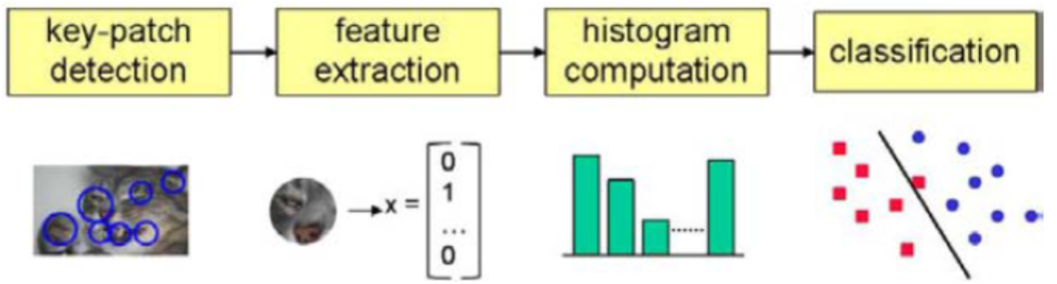
\includegraphics[width=0.7\linewidth]{_images/stepsSVM}
				\caption{BoW Pipeline}
				\label{fig:stepssvm}
			\end{figure}
			\item The second system will make use of Neural Network, namely a CNN.
		\end{enumerate}
	
		\item \underline{The Features:}\\
		You will use these features:
		\begin{enumerate}[a.]
			\item Shi-Tomasi corner detector
			\item HoG (Histogram of Gradients)
		\end{enumerate}
		These are popular feature descriptors available online and in OpenCV.\\
		\underline{The Classifier:} Use a Support Vector Machine (SVM). Look for a library (one is given 
		at the end of this document) and learn how to use it.
		\item THE DATASET AND DATA PREPARATION:\\
		\begin{enumerate}[a.]
			\item Choose one task from:
			\begin{itemize}
				\item \href{https://data.mendeley.com/datasets/hb74ynkjcn/1}{Leaf dataset}
				\item \href{https://github.com/yalesong/natops}{Aircraft signal dataset}
			\end{itemize}
			\item Read the images and assign their corresponding labels.
			\begin{itemize}
				\item Consider  that  the  images  are  at  different  sizes,  you  must  transform  all 
				images to the same size.
				\item Colored  pictures  may  have  to  be  transformed  to  black  and  white  (bag  of 
				features).
				\item Usually  images  are  not  normalized  regarding  contrast,  if  needed  this  can 
				be done easily with just one line of code such as (this is Matlab):\\
				\verb|img2 = uint8((double(img)-double(min(min(img))))*(255/|\\
				\verb|double(max(max(img))-min(min(img)))));|
			\end{itemize}
		\end{enumerate}
		\item BAG  OF  FEATURES.  OBJECT  REPRESENTATION:
		  feature  extraction  using  Shi-
		Tomasi/HoG.
		\begin{enumerate}[a.]
			\item After  the  keypoint  localization,  you  have  to  convert  them  into  their  feature 
			vectors.
			\item Those  feature  vectors  must  be  clustered  into  a  histogram,  for  this  the  most  used 
			method is k-means (available in OpenCV: MiniBatchKMeans).
		\end{enumerate}
		\item LEARNING: Training a classifier. Download the code for a classifier. You will use an 
		SVM  (e.g.  library  libsvm  for  Python  or  any  other  one).  For  comparison  you  will 
		adapt the code of CNN explained in class, but replace VGG for Resnet-18. The CNN 
		must  also  be  adapted  to  work  with  your  dataset.  For  the  CNN  you  do  not  need  to 
		create  a  histogram,  just  feed  the  images  to  the  CNN  and  record  the  accuracy  and 
		confusion matrix. Remember to use data augmentation.
		\item RECOGNITION: Using classifier in test data. We have now a trained system that can 
		distinguish an image (leaf type, aircraft sign).
		\item RESULTS\\
		At  this  point  we  have  a  classification  system  that  can  recognize  what  is  on  the 
		picture. We have to measure how good is our system, for this we compare the true 
		labels  of  the  test  set  with  the  ones  obtained  in  step  5. The  higher  the  percentage 
		the  better,  if  you  have  2  classes  and  this  percentage  is  below  50\%  it  means  our 
		system is ever worse than using chance (a coin with tails and heads), if it is a bit 
		over 50\% it means it is ok, 70-80\% good enough and over 90\% quite good, if over 
		95\% it is great. Other cases: if you have 10 classes, you should get over 10\%.\\
		Create  first  a  confusion  matrix,  from  this,  you  can  build  a  table  reporting  true 
		positives, false positives, true negatives and false negatives.\\
		Compare  the  three  features  for  the  two  classifiers  (Bag  of  words  with  SVM  and 
		CNN): Shi-tomasi, HoG to see which one performs better at the task. This should 
		be reported in graphs, tables or ROC curves
	\end{enumerate}
\newpage
\section{Preliminary}
This document and the code has been done on my own. I shared the code and the images for the BoW/SVM part with Ori Sofer, therefore there will be similarities.



\section{Introduction on object recognition and steps to it}
A very big and also important part of computer vision is object recognition. Object recognition can also be sectioned into object recognition, where we want to identify the class of an object. And into instance recognition where we want to identify one instance of a class, for example a human face should be used for unlocking a computer, of course we don't want anyone to be able to unlock the computer. In this assignment general object recognition is pursued. There is also a significant difference between recognizing one object class (or instance) or multiple objects.
There are several approaches to object recognition. The simplest being a Bag-of-Words approach. This technique originates in the area of natural language processing.\\
The steps for BoW:\\
\begin{enumerate}
	\item Detect key points.
	\item Generate feature vectors of the detected key points
	\item Using k-means clustering find clusters and count the number of occurrences (histogram computation).
	\item With the help of a neural network or a support vector machine, try to discriminate the classes from each other.
\end{enumerate}

This usually works pretty good and is fast and simple compared to other methods.
One of these other methods is a parts-based representation approach.

This approach tries to cope with a problem that arises with the BoW approach. That is, location of the found features and their correspondence isn't taken into account which means that there could be parts (or rather features) which can be found all over the image but the resulting class has a completely different structure.
With the parts-based approach, objects are build of parts that have a certain location in respect to each other. But this is not easy as the relational position cannot be fixed as for example faces differ from each person to another. Also partial occlusion has to be dealt with which is also a hard problem.

Another way to get to object recognition is using a convolutional neural network. This is a very sophisticated approach that can work very accurate. A CNN consists of convolutional layers as the name suggests. These layers apply a trainable filter to the images in a convolutional fashion, shown in equation \ref{conv_eq}. In this equation g is the convolved image, f is the input image and h is the filter.

\begin{align}\label{conv_eq}
	g(x,y) = \sum_j \sum_k f(x-j, y-k) * h(j, k)
\end{align} 

The result of the first layer is similar to applying a gabor filter, therefore is able to detect edges. With more convolutional layers the extractable information is much more complex for example structural information can be extracted.
After the convolutional layer normaly a fully connected feed forward neural network is used to discriminate the classes. A softmax function is applied to the output to have exactly one class as output. 



\section{Purpose/Hypothesis}
The purpose of all of this is to evaluate for one the performance of two different Bag-of-Words approaches. First one using Shi-Tomasi edge detector to find key points and another one using a Histogram-of-Gradients approach. And another approach using a CNN. The results should then be evaluated and interpreted.
I hypothesize that the CNN will be performing better than the SVM approaches as it is much more sophisticated.





\newpage
\section{Approach and Implementation}
\subsection{Data}
I decided to use the leafs dataset provided further above in the instructions. The plant classes are divided into healthy and diseased, I used both for training and testing of the object classification approaches. There is a strong bias in the data for example to plant class Jamun (P5) as there are 624 images (in healthy and diseased) opposing to Bael (P4) which has only 118 images, where all of them are diseased. To prevent a bias also in the machine learning model data augmentation has been used. I generated so many images that there were 1000 per class. To have more variance of the leafs in the images I used at least one of the following transformations
\begin{itemize}
	\item flip
	\item rotate by 0 to 360\textdegree (with 90\textdegree steps)
	\item darken or brighten
	\item changing the contrast
	\item increase or decrease the image saturation
	\item or scale by 10\% and crop it
\end{itemize}
This worked out pretty good. Two classes Basil (P8) and the previously mentioned Bael (P4) class contained just healthy and diseased images respectively. For these classes I've decided to just generate 1000 images within the categories that were available.

\subsection{SVM/BoW}
\textbf{General}\\
All of the aforementioned steps have to be run through and are practically the same for both Shi-Tomasi and HoG. To use a zip as input and not having to unpack the entire zip I've used the zipfile library in python. The code has been reused to a great part from last semesters project from the Visual Computing PS. 
The steps can be roughly described as:
\begin{enumerate}
	\item Load files contained in zip.
	\item Encode the classes to integers from 0 to 11.
	\item Load all the images into memory.
	\item Now extract feature vectors from all images.
	\item Calculate $ \text{number of classes} * 10$ clusters of the feature vector space.
	\item Calculate distance of each feature vector of each image to closest cluster.
	\item Split files into train and test data (80\% for training).
	\item Train SVM using the test data.
	\item Evaluate the performance of the trained SVM.
	\item Save the SVM parameters.
\end{enumerate}
\textbf{Shi-Tomasi}\\
As Shi-Tomasi is just a corner detection algorithm we have to use another algorithm that helps us generating a feature vector for each found key point. I've decided to use SIFT for this as I am already familiar with it. As SIFT uses instances of the class cv.KeyPoint instead of simple image coordinates, because it can hold other useful information like size and magnitude. Therefore I had to wrap it.
All further steps are the same as for HoG.\\\\
\textbf{HoG}\\
HoG is pretty straight forward compared to Shi-Tomasi. At first we have to resize the images to a lower resolution as the memory demand of HoG is drastically greater than the other approach. After that we create a HoGDescriptor instance which we then apply to each image. All further steps are again the same as described in the General section above.

\subsection{CNN}
For the CNN I've used large parts of the provided Jupyter Notebook. But before training was even possible I had to write a custom dataset class to access the data of the zip and get the correct class names. This worked in a similar way to the BoW approach dataloader. 
Then the train- and test-dataloaders are set up with again the splitted files (this is being randomized), the dataloaders were set up with a batch size of 10 images.
Now the ResNet18 model is loaded, and we freeze all layers. I added a few layers to the fully connected part of the network.
Also I used kaiming initialization to hopefully start from better values for training. After that the criterion and the the optimizer are defined. I used Adam with a learning rate of $0.001$ and a weight decay rate of $0.0001$. 
Then the neural network is trained for 20 epochs, evaluated and saved afterwards.



\newpage
\section{Results}
\subsection{BoW - Shi-Tomasi}
For Shi-Tomasi I tried to change various parameters like maxCorners, qualityLevel, minDistance and blockSize also I used a gridsearch approach to optimize the SVM training.\\
The best results were achieved by using a high number of maxCorners $\ge 800$ a low quality level $\le 0.00001$ as well as a low minDistance $\le 3$ between found corners and a block size of $15$ as parameters for Shi-Tomasi.

The best SVM parameters were the kernel CHI2, C didn't seem to affect the result as much best were between $1,000 - 10,000$. Also $\gamma$ didn't seem to have a large impact therefore I used the default value of $1$. The termination criteria has been set to $5,000,000$ iterations which seemed to be large enough, but also required quite a long time for fitting the SVM to the data.

Also the input images have been resized to 1024x1024 as otherwise it uses too much memory. I've also applied a Gaussian filter of size 7x7 to remove some of that noise.
\\\\
\textbf{Accuracy}\\
The combined Shi-Tomasi+SIFT SVM achieved a respectable accuracy of 85.875\%.\\\\
\textbf{Confusion Matrix}\\
\begin{figure}[H]
	\centering
	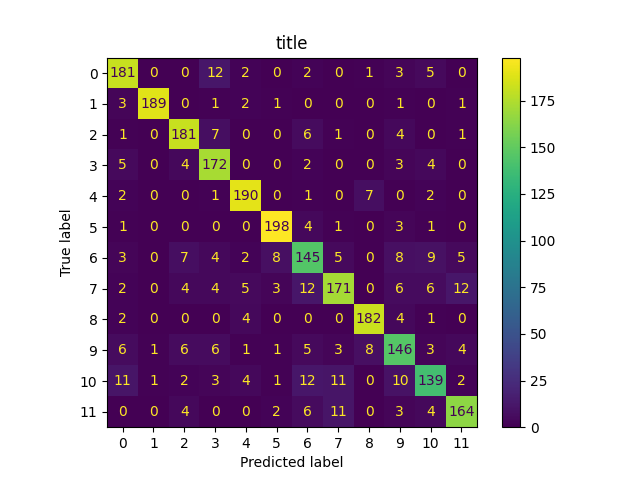
\includegraphics[width=0.7\linewidth]{_images/ShiTomasiConfusionMat}
	\caption{Confusion matrix Shi-Tomasi+SIFT.}
	\label{fig:shitomasiconfusionmat}
\end{figure}
It is visible from the matrix that most predictions are pretty accurate due to the highest values being on the diagonal. There are some outliers like for example class 10 being detected as class 6 or 7. I missed to replace the class numbers with the labels and just saw this as of writing (same for HoG).


\subsection{BoW - HoG}
For HoG I wasn't able to find such good suiting parameters as for the Shi-Tomasi+SIFT SVM. Nevertheless the best combination for HoG was using a winSize of 128x128 a blockSize of 16x16 a blockStride of 4x4 (anything less wouldn't work as it required loads of main memory) cellSize 8x8 (also the same here, less would not be possible) and nbins of size 9.\\
The SVM parameters I used were the same as for the Shi-Tomasi implementation. I tried many different values and the variance wasn't as large as for the Shi-Tomasi. So different kernels were much closer to the best performance. To be precise the kernels CHI2, RBF and SIGMOID performed very similar.\\
\\\textbf{Accuracy}\\
The HoG SVM achieved the worst performance of the bunch with an accuracy of 65.625\%.\\\\
\textbf{Confusion Matrix}
\begin{figure}[H]
	\centering
	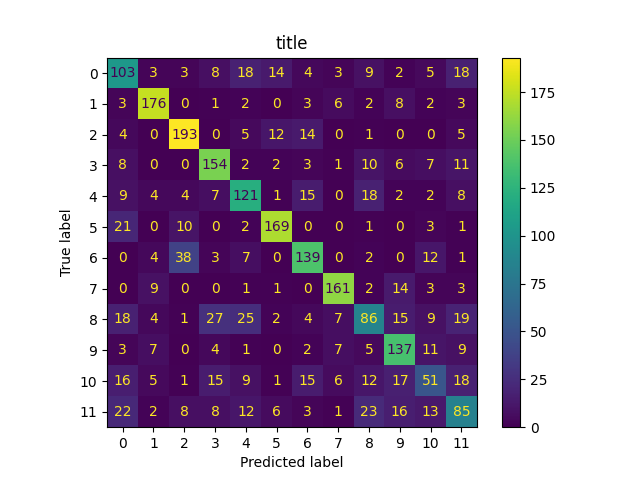
\includegraphics[width=0.7\linewidth]{_images/HoGConfusionMat}
	\caption{Confusion Matrix}
	\label{fig:hogconfusionmat}
\end{figure}
Compared to the first confusion matrix \ref{fig:shitomasiconfusionmat} here are much more outliers with the maximum being 38 for the true class 6 and predicted 2. This is 18.4\% of the entire class not counting all other outliers, that would sum up to over 32\%. It is quite obvious that this classifier does not perform good.
\newpage
\subsection{CNN}
This CNN is build upon ResNet-18 which looks like the following:
\begin{figure}[H]
	\centering
	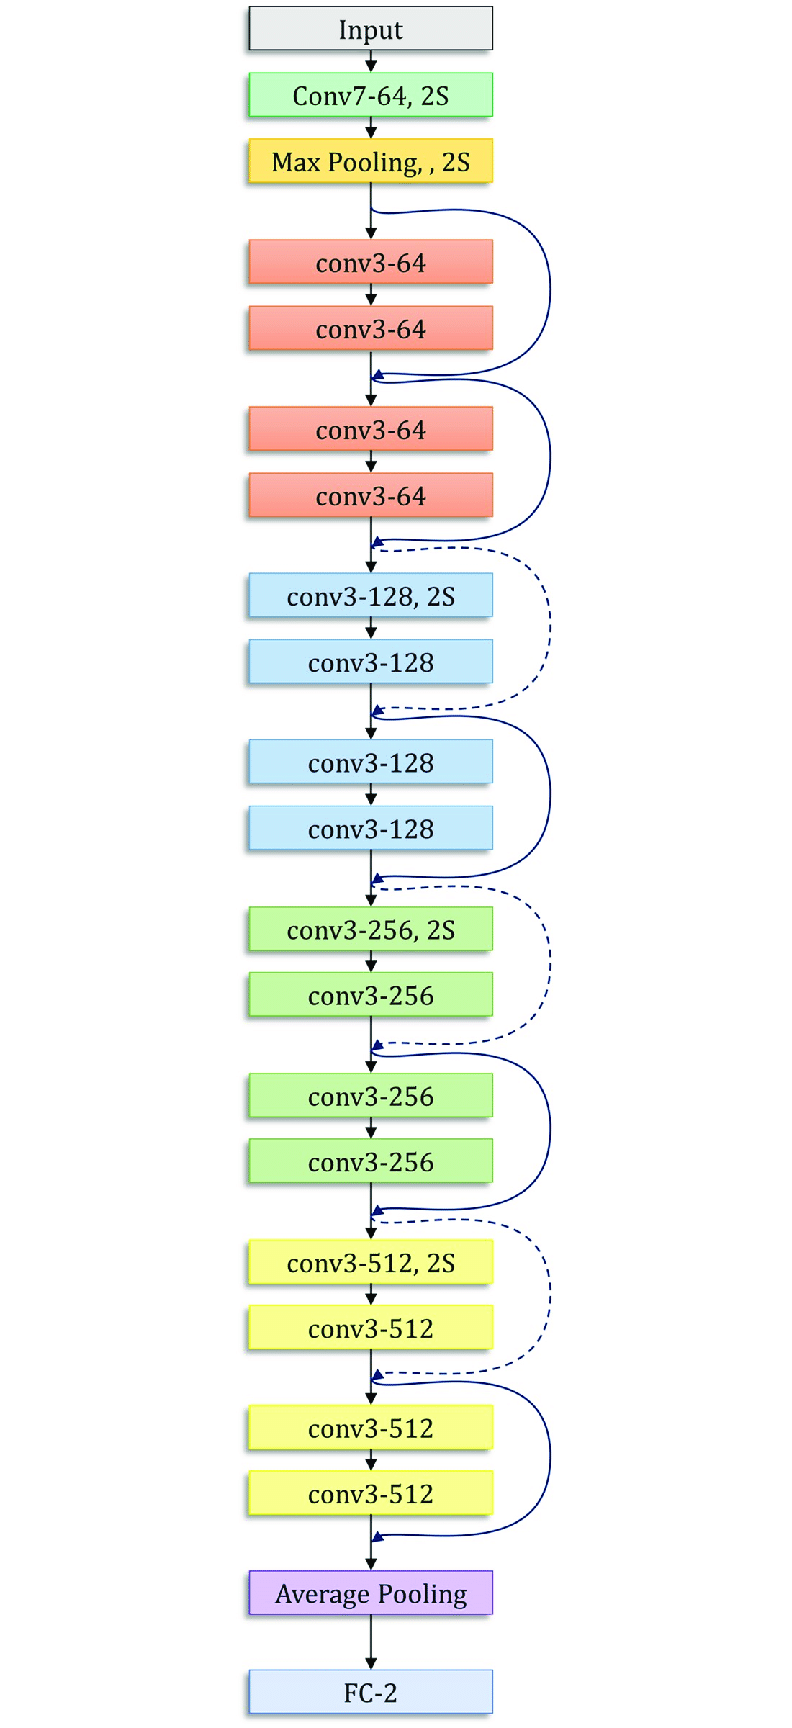
\includegraphics[width=0.25\linewidth]{_images/resnetArch}
	\caption{ResNet-18 Source:  \href{https://www.researchgate.net/figure/Architecture-of-the-ResNet-18-model-used-in-this-study_fig3_354432343}{Researchgate}}
	\label{fig:resnetarch}
\end{figure}

To get ResNet working with our leaf dataset I replaced the default fully connected layers at the end and froze the convolutional layers as they were pretrained and hopefully would be able to detect all relevant information.
The output of the convolutional layer part is a vector of length 512, therefore the fc part must have such an input. And as we have 12 classes the output must be of length 12 too. I decided to add a few layers, 6 to be precise, in between to cope with all the information better (structure can be seen below in the Appendix).\\\\
The CNN performed good after just 10 epochs with about 84\% accuracy, but I decided to train for 20 epochs which yielded a very good 95\% accuracy. 

\begin{figure}[H]
	\centering
	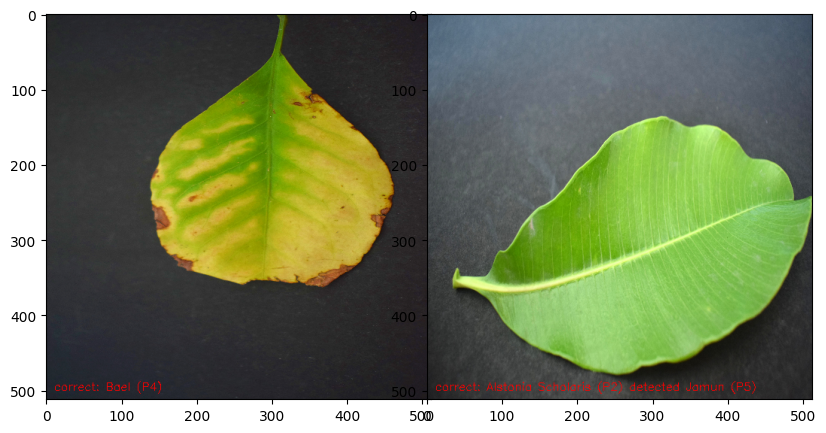
\includegraphics[width=0.6\linewidth]{_images/CNNcorrect_falseImg2}
	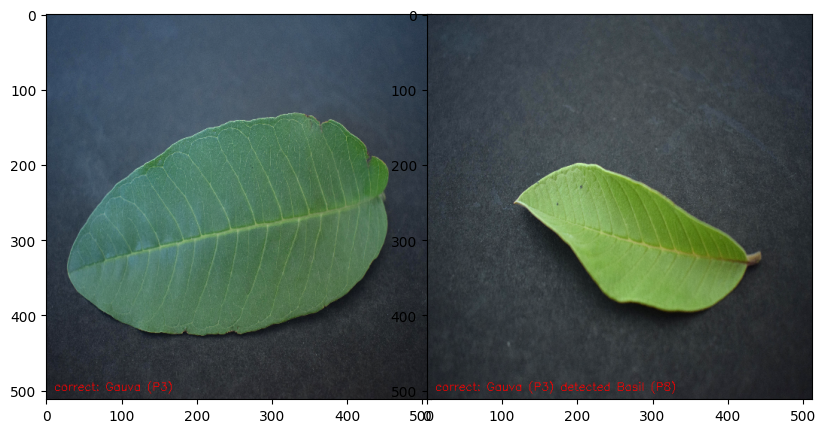
\includegraphics[width=0.6\linewidth]{_images/CNNcorrect_falseImg}
	\caption{Example images of correct classified images and false ones on the right (with the wrong class and the correct one).}
	\label{fig:cnncorrectfalseimg2}
\end{figure}

\textbf{Confusion Matrix}
\begin{figure}[H]
	\centering
	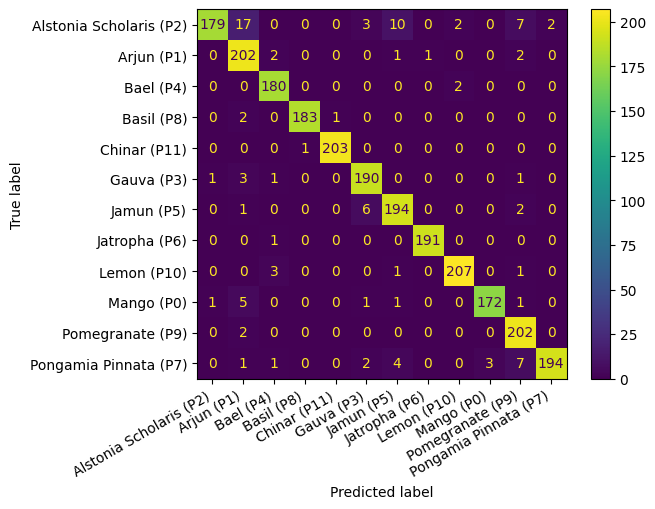
\includegraphics[width=0.7\linewidth]{_images/CNNConfusionMat}
	\caption{Confusion matrix of the CNN classification.}
	\label{fig:cnnconfusionmat}
\end{figure}
In the confusion matrix we can observe looking at the diagonal that most of the images have a very good classification. The worst performance is on the class Alstonia Scholaris (P2) which has been misclassified the most often (as Arjun (P1) and Jamun (P5)).\\

\textbf{ROC Curve}
The ROC curve has 'only' been represented using 400 datapoints as it requires very much memory. I tried to use swap as I was only able to use 150 points at first before 32 GB of memory were full. 400 still used about 60 gigabytes of memory.

\begin{figure}[H]
	\centering
	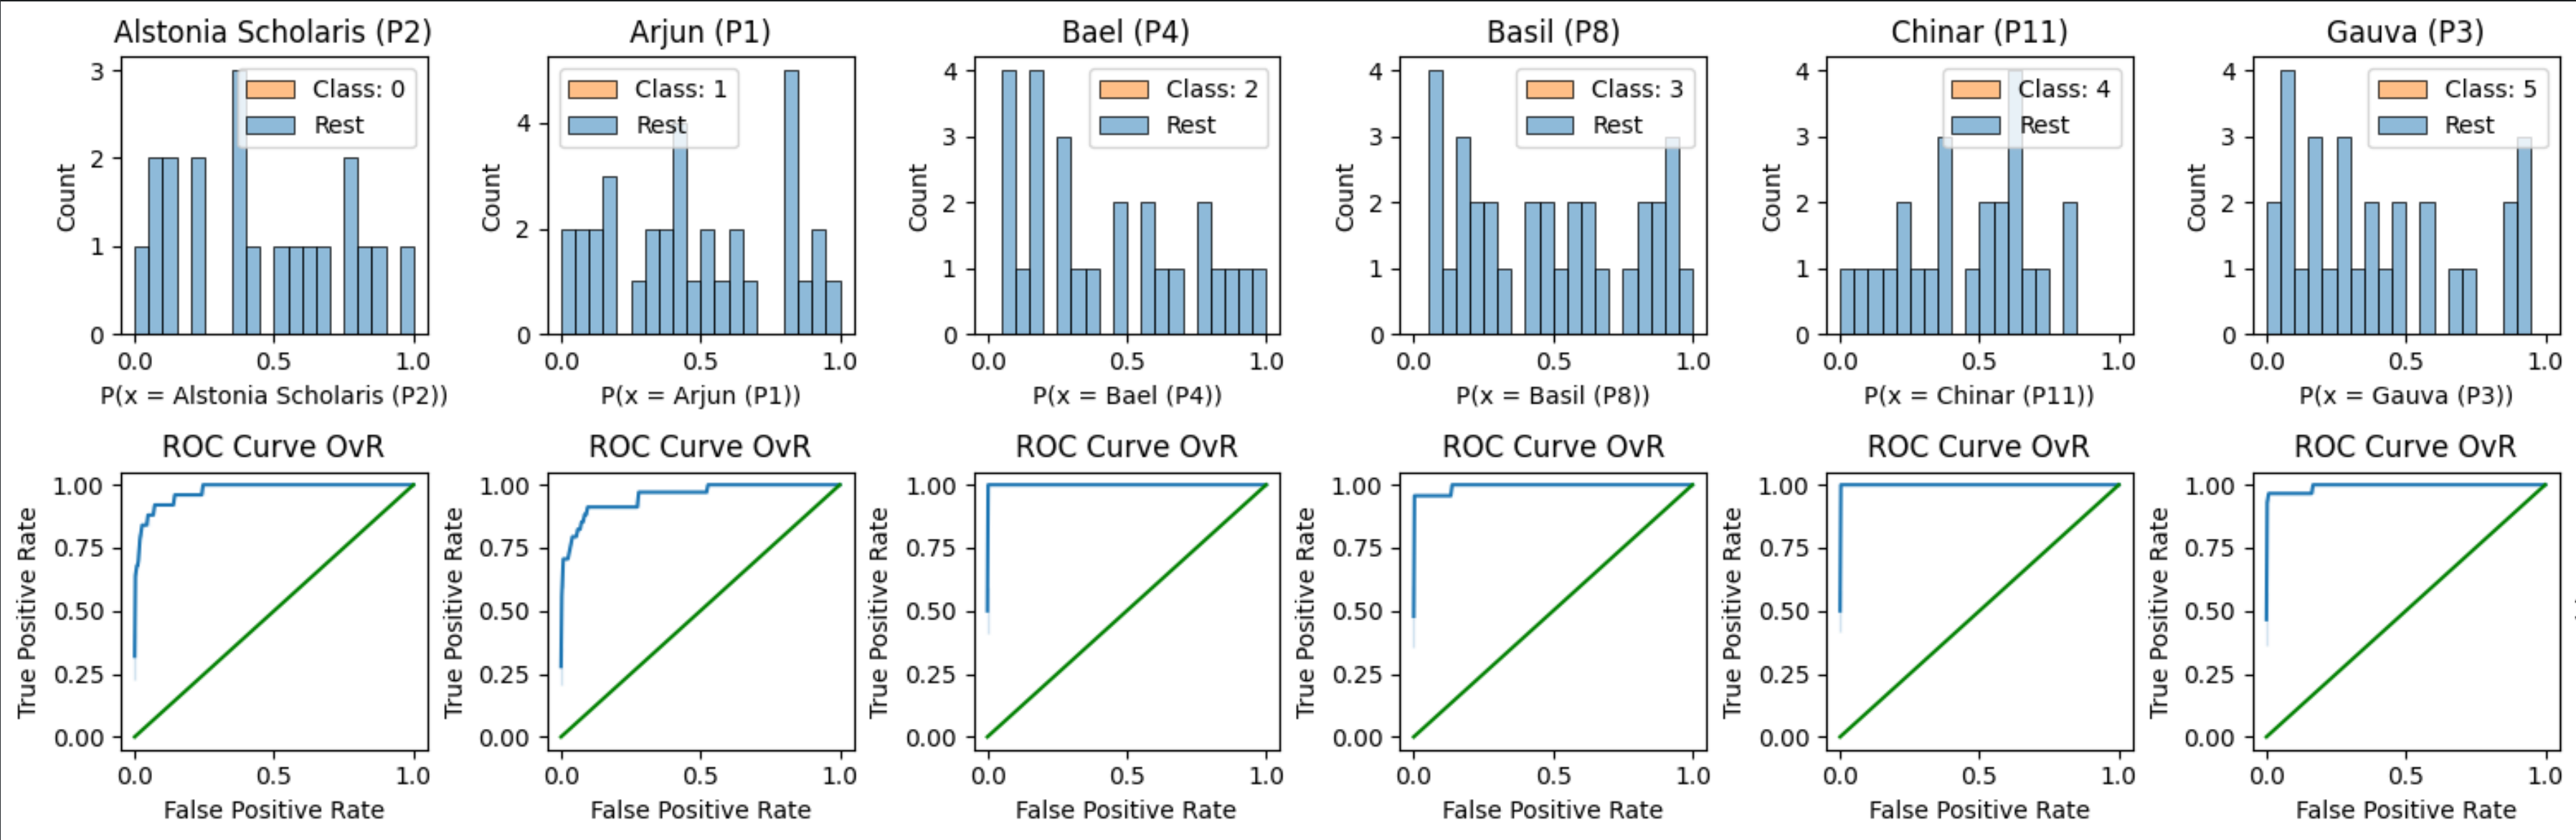
\includegraphics[width=0.7\linewidth]{_images/CNNroccurve450part1}
	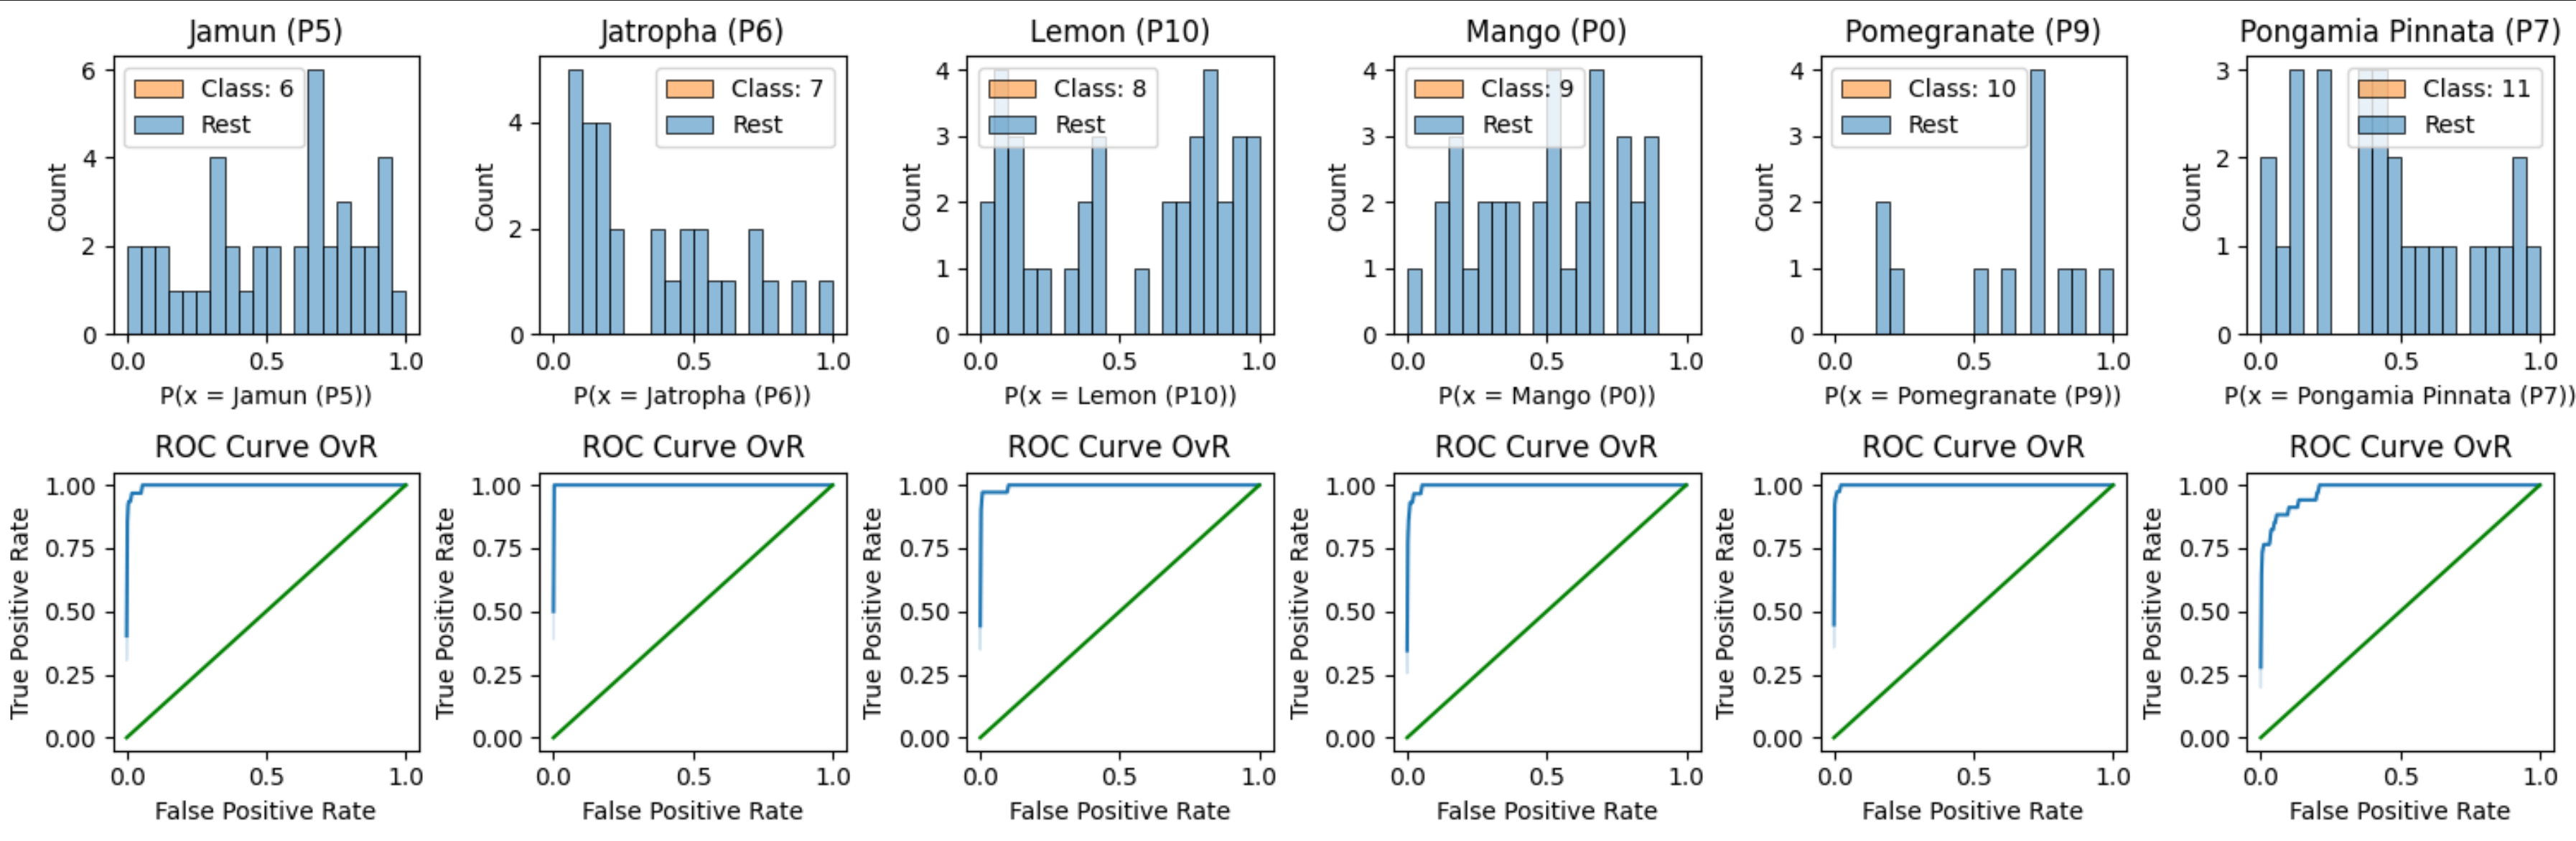
\includegraphics[width=0.7\linewidth]{_images/CNNroccurve450part2}
	\caption{ROC curves for each class (One-vs-Rest).}
	\label{fig:cnnroccurve450}
\end{figure}
From the ROC curves can be seen that for most of the classes the performance is good or even very good and for some classes, e.g. Alstonia Scholaris (P2) the area under the curve isn't as much. This data has to be interpreted with caution as just a part of the data has been used, therefore it isn't representative.

\begin{center}
\begin{tabular}{|c|c|c|c|c|}
	\hline
	Class & TN & FP & FN & TP \\
	\hline
	Alastonia Scholaris & 79326 & 69474 & 474 & 10726 \\
	\hline
	Arjun & 78863 & 69537 & 937 & 10663 \\
	\hline
	Bael & 78932 & 64268 & 868 & 15932 \\
	\hline
	Basil & 79180 & 67220 & 620 & 12980 \\
	\hline
	Chinar & 79365 & 68635 & 435 & 11565 \\
	\hline
	Gauva & 79164 & 69236 & 636 & 10964 \\
	\hline
	Jamun & 79007 & 64993 & 793 & 15207 \\
	\hline
	Jatropha & 79019 & 64981 & 781 & 15219 \\
	\hline
	Lemon & 79500 & 70500 & 300 & 9700 \\
	\hline
	Mango & 79003 & 65397 & 797 & 14803 \\
	\hline
	Pomegranate & 79302 & 67898 & 498 & 12302 \\
	\hline
	Pongamia Pinnata & 79048 & 68152 & 752 & 12048 \\
	\hline
\end{tabular}
\end{center}



\newpage
\section{Discussion}
What  you  learnt  about  this  assignment  and  how  the  method  can  be  improved  or 
extended.\\\\
I learned a bit more about using OpenCV (especially at the augmentation part) and their implementation of LibSVM. Also I learned a bit more about using ResNet with PyTorch and some quirks with Torch as I used it on two systems my computer with a GPU and my laptop without a GPU and especially the juggling around with the memory location of objects.\\
I liked this assignment, there was just a bit of trouble with visualizing the ROC curves thats also a reason why I just did it for the CNN. Maybe a bit more time would be nice, as this entire exercise was joined by some exams.

\newpage
\section{Appendix}
The code has been handed in seperately as it is a Jupyter Notebook for one and all of the BoW is distributed over several files.





\newpage
\textbf{CNN - Structure}
\begin{center}
	\begin{tabular}{|c|c|c|c|}
		\hline
		Layer number &         Layer (type)   &     Output Shape   &   Param \# \\
		\hline
		\hline
		1 &             Conv2d-1   & [-1, 64, 16, 16]   & 9408 \\
		\hline
		2 &        BatchNorm2d-2   & [-1, 64, 16, 16]   & 128 \\
		\hline
		3 &               ReLU-3   & [-1, 64, 16, 16]   & 0 \\
		\hline
		4 &          MaxPool2d-4   &   [-1, 64, 8, 8]   & 0 \\
		\hline
		5 &             Conv2d-5   &   [-1, 64, 8, 8]   & 36864 \\
		\hline
		6 &        BatchNorm2d-6   &   [-1, 64, 8, 8]   & 128 \\
		\hline
		7 &               ReLU-7   &   [-1, 64, 8, 8]   & 0 \\
		\hline
		8 &             Conv2d-8   &   [-1, 64, 8, 8]   & 36864 \\
		\hline
		9 &        BatchNorm2d-9   &   [-1, 64, 8, 8]   & 128 \\
		\hline
		10 &              ReLU-10   &   [-1, 64, 8, 8]   & 0 \\
		\hline
		11 &        BasicBlock-11   &   [-1, 64, 8, 8]   & 0 \\
		\hline
		12 &            Conv2d-12   &   [-1, 64, 8, 8]   & 36864 \\
		\hline
		13 &       BatchNorm2d-13   &   [-1, 64, 8, 8]   & 128 \\
		\hline
		14 &              ReLU-14   &   [-1, 64, 8, 8]   & 0 \\
		\hline
		15 &            Conv2d-15   &   [-1, 64, 8, 8]   & 36864 \\
		\hline
		16 &       BatchNorm2d-16   &   [-1, 64, 8, 8]   & 128 \\
		\hline
		17 &              ReLU-17   &   [-1, 64, 8, 8]   & 0 \\
		\hline
		18 &        BasicBlock-18   &   [-1, 64, 8, 8]   & 0 \\
		\hline
		19 &            Conv2d-19   &  [-1, 128, 4, 4]   & 73728 \\
		\hline
		20 &       BatchNorm2d-20   &  [-1, 128, 4, 4]   & 256 \\
		\hline
		21 &              ReLU-21   &  [-1, 128, 4, 4]   & 0 \\
		\hline
		22 &            Conv2d-22   &  [-1, 128, 4, 4]   & 147456 \\
		\hline
		23 &       BatchNorm2d-23   &  [-1, 128, 4, 4]   & 256 \\
		\hline
		24 &            Conv2d-24   &  [-1, 128, 4, 4]   & 8192 \\
		\hline
		25 &       BatchNorm2d-25   &  [-1, 128, 4, 4]   & 256 \\
		\hline
		26 &              ReLU-26   &  [-1, 128, 4, 4]   & 0 \\
		\hline
		27 &        BasicBlock-27   &  [-1, 128, 4, 4]   & 0 \\
		\hline
		28 &            Conv2d-28   &  [-1, 128, 4, 4]   & 147456 \\
		\hline
		29 &       BatchNorm2d-29   &  [-1, 128, 4, 4]   & 256 \\
		\hline
		30 &              ReLU-30   &  [-1, 128, 4, 4]   & 0 \\
		\hline
		31 &            Conv2d-31   &  [-1, 128, 4, 4]   & 147456 \\
		\hline
		32 &       BatchNorm2d-32   &  [-1, 128, 4, 4]   & 256 \\
		\hline
		33 &              ReLU-33   &  [-1, 128, 4, 4]   & 0 \\
		\hline
		34 &        BasicBlock-34   &  [-1, 128, 4, 4]   & 0 \\
		\hline
		35 &            Conv2d-35   &  [-1, 256, 2, 2]   & 294912 \\
		\hline
		36 &       BatchNorm2d-36   &  [-1, 256, 2, 2]   & 512 \\
		\hline
		37 &              ReLU-37   &  [-1, 256, 2, 2]   & 0 \\
		\hline
		38 &            Conv2d-38   &  [-1, 256, 2, 2]   & 589824 \\
		\hline
		39 &       BatchNorm2d-39   &  [-1, 256, 2, 2]   & 512 \\
		\hline
		40 &            Conv2d-40   &  [-1, 256, 2, 2]   & 32768 \\
		\hline
		41 &       BatchNorm2d-41   &  [-1, 256, 2, 2]   & 512 \\
		\hline
		42 &              ReLU-42   &  [-1, 256, 2, 2]   & 0 \\
		\hline
		43 &        BasicBlock-43   &  [-1, 256, 2, 2]   & 0 \\
		\hline
		44 &            Conv2d-44   &  [-1, 256, 2, 2]   & 589824 \\
		\hline
		45 &       BatchNorm2d-45   &  [-1, 256, 2, 2]   & 512 \\
		\hline
		46 &              ReLU-46   &  [-1, 256, 2, 2]   & 0 \\
		\hline
		47 &            Conv2d-47   &  [-1, 256, 2, 2]   & 589824 \\
		\hline
		48 &       BatchNorm2d-48   &  [-1, 256, 2, 2]   & 512 \\
		\hline
		49 &              ReLU-49   &  [-1, 256, 2, 2]   & 0 \\
		\hline
		50 &        BasicBlock-50   &  [-1, 256, 2, 2]   & 0 \\
		\hline
	\end{tabular}
	\newpage
	
	\begin{tabular}{|c|c|c|c|}
		\hline
		Layer number &         Layer (type)   &     Output Shape   &   Param \# \\
		\hline
		\hline
		51 &            Conv2d-51   &  [-1, 512, 1, 1]   & 1179648 \\
		\hline
		52 &       BatchNorm2d-52   &  [-1, 512, 1, 1]   & 1024 \\
		\hline
		53 &              ReLU-53   &  [-1, 512, 1, 1]   & 0 \\
		\hline
		54 &            Conv2d-54   &  [-1, 512, 1, 1]   & 2359296 \\
		\hline
		55 &       BatchNorm2d-55   &  [-1, 512, 1, 1]   & 1024 \\
		\hline
		56 &            Conv2d-56   &  [-1, 512, 1, 1]   & 131072 \\
		\hline
		57 &       BatchNorm2d-57   &  [-1, 512, 1, 1]   & 1024 \\
		\hline
		58 &              ReLU-58   &  [-1, 512, 1, 1]   & 0 \\
		\hline
		59 &        BasicBlock-59   &  [-1, 512, 1, 1]   & 0 \\
		\hline
		60 &            Conv2d-60   &  [-1, 512, 1, 1]   & 2359296 \\
		\hline
		61 &       BatchNorm2d-61   &  [-1, 512, 1, 1]   & 1024 \\
		\hline
		62 &              ReLU-62   &  [-1, 512, 1, 1]   & 0 \\
		\hline
		63 &            Conv2d-63   &  [-1, 512, 1, 1]   & 2359296 \\
		\hline
		64 &       BatchNorm2d-64   &  [-1, 512, 1, 1]   & 1024 \\
		\hline
		65 &              ReLU-65   &  [-1, 512, 1, 1]   & 0 \\
		\hline
		66 &        BasicBlock-66   &  [-1, 512, 1, 1]   & 0 \\
		\hline
		67 & AdaptiveAvgPool2d-67   &  [-1, 512, 1, 1]   & 0 \\
		\hline
		68 &            Linear-68   &        [-1, 400]   & 205200 \\
		\hline
		69 &         LeakyReLU-69   &        [-1, 400]   & 0 \\
		\hline
		70 &            Linear-70   &        [-1, 300]   & 120300 \\
		\hline
		71 &         LeakyReLU-71   &        [-1, 300]   & 0 \\
		\hline
		72 &            Linear-72   &        [-1, 200]   & 60200 \\
		\hline
		73 &         LeakyReLU-73   &        [-1, 200]   & 0 \\
		\hline
		74 &            Linear-74   &        [-1, 100]   & 20100 \\
		\hline
		75 &         LeakyReLU-75   &        [-1, 100]   & 0 \\
		\hline
		76 &            Linear-76   &         [-1, 50]   & 5050 \\
		\hline
		77 &         LeakyReLU-77   &         [-1, 50]   & 0 \\
		\hline
		78 &            Linear-78   &         [-1, 12]   & 612 \\
		\hline
	\end{tabular}
\end{center}
\end{document}






















